\subsubsection{Fractionally Differentiated Features}

Standard stationarity transformations (i.e. integer differentiation) reduce signal by removing memory. Although stationarity is necessary for inferential purposes, it is rarely the case that we want all memory to be erased.\\
Fractionally differentiated processes exhibit long-term persistence and anti-persistence, hence enhancing the forecasting power compared to standard ARIMA approach.

\begin{definition} \hlt{BackShift Operator}\\
Let $B$ be the backshift operator applied to a matrix of real-valued features $\{X_t \}$, where $B^k X_t = X_{t-k}$ for any integer $k \geq 0$. By binomial expansion, we then have
\begin{align}
(1-B)^d = \sum\limits_{k=0}^{\infty} \binom{d}{k} (-B)^k &= \sum\limits_{k=0}^{\infty} \prod\limits_{i=0}^{k-1} (d-i) \frac{(-B)^k}{k!} \nonumber \\
&= \sum\limits_{k=0}^{\infty} (-B)^k \prod\limits_{i=0}^{k-1} \frac{d-i}{k-i} \nonumber \\
&= 1 - dB + \frac{d(d-1)}{2!} B^2 - \frac{d(d-1)(d-2)}{3!} B^3 + \cdots \nonumber 
\end{align}
\end{definition}

\begin{remark}
\label{rmk:propfracdifffeat} 
\hlt{Properties of Fractionally Differentiated Features}\\
Let $d$ be a real (non-integer) positive number. The arithmetic series consists of dot product
\begin{align}
\tilde{X}_t &= \sum\limits_{k=0}^{\infty} \omega_k X_{t-k} \nonumber \\
\omega &= \left\{ 1, -d, \frac{d(d-1)}{2!}, - \frac{d(d-1)(d-2)}{3!}, \ldots, (-1)^k \prod\limits_{i=0}^{k-1} \frac{d-1}{k!}, \ldots \right\} \nonumber \\
X &= \{X_t, X_{t-1}, \ldots, X_{t-k}, \ldots \} \nonumber
\end{align}
where $\omega$ are the weights, $X$ are the values. Properties of these features are:
\begin{enumerate}[label=\roman*.]
\setlength{\itemsep}{0pt}
\item Long memory: if $d$ is a positive integer number, then
\begin{equation}
\prod\limits_{i=0}^{k-1} \frac{d-i}{k!} = 0 \ \ \forall > d \nonumber
\end{equation}
and memory beyond that point is cancelled.
\item Iterative weight generation: given sequence of weights $\omega$, for $k = 0, \ldots, \infty$, the weights are
\begin{equation}
\omega_k = - \omega_{k-1} \frac{d - k + 1}{k}, \ \ \ \omega_0 = 1 \nonumber
\end{equation}
\item Convergence: For $k > d$, if $\omega_{k-1} \neq 0$, then
\begin{equation}
\abs{\frac{\omega_{k}}{\omega_{k-1}}} = \abs{\frac{d-k+1}{k}} < 1 \nonumber
\end{equation}
and $\omega_k = 0$ otherwise. Hence weights converge asymptotically to zero.\\
For positive $d$ and $k < d+1$, then $\frac{d-k+1}{k} \geq 0$, which makes initial weights alternate in sign.\\
For non-integer $d$, once $k \geq d+1$, $\omega_k$ will be negative if int$[d]$ is even, and positive otherwise.\\
In summary, $\lim_{k \rightarrow \infty} = 0^-$ when int$[d]$ is even, and $\lim_{k \rightarrow \infty} = 0^+$ when int$[d]$ is odd.\\
In special case $d \in (0,1)$, that $-1 < \omega_k < 0 \ \forall k > 0$. Alternate weight signs makes $\{\tilde{X}_t \}_{t = 1, \ldots, T}$ stationary, as memory wanes or is offset over the long run.
\end{enumerate}
\end{remark}

\begin{figure}[H]
\centering
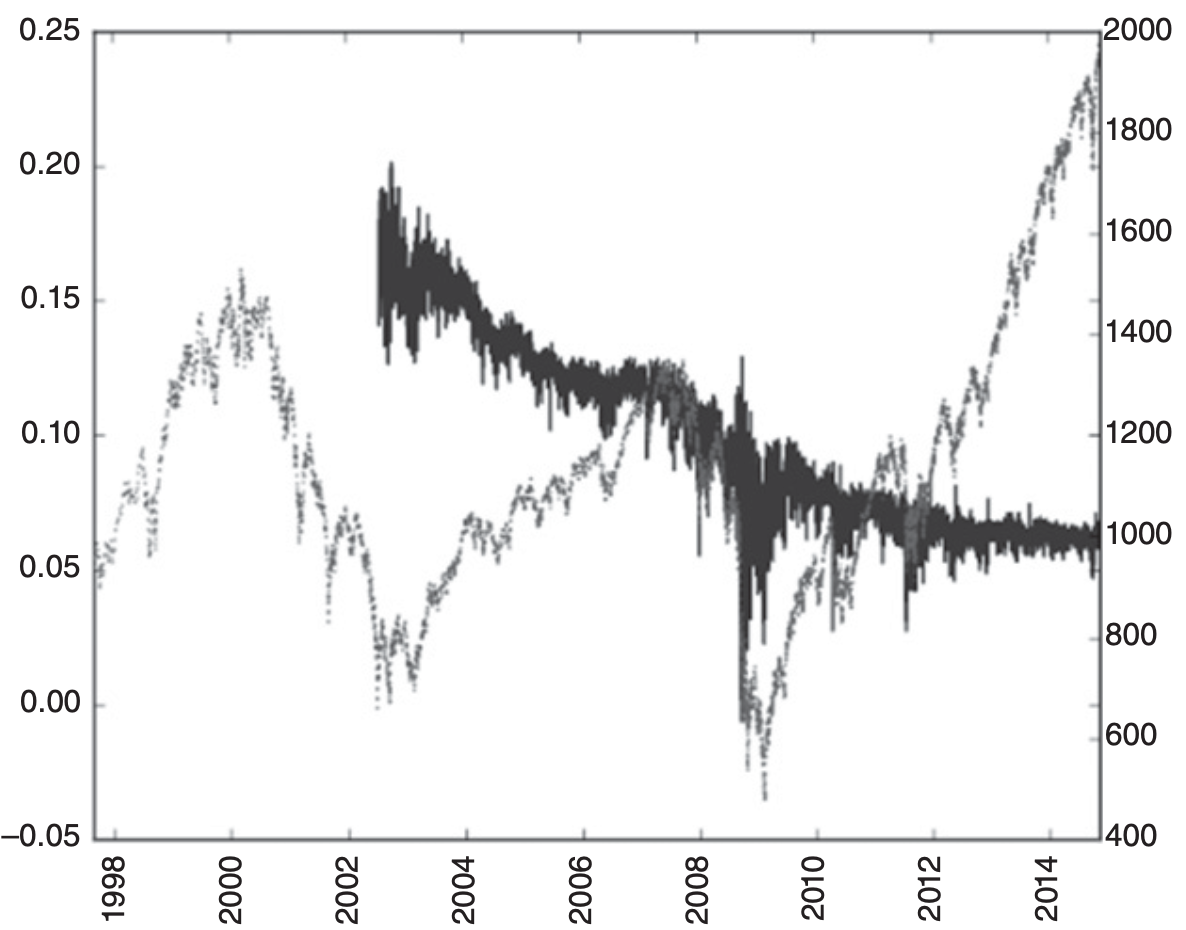
\includegraphics[scale=0.32]{/intro/fracdiffexpandwindow}
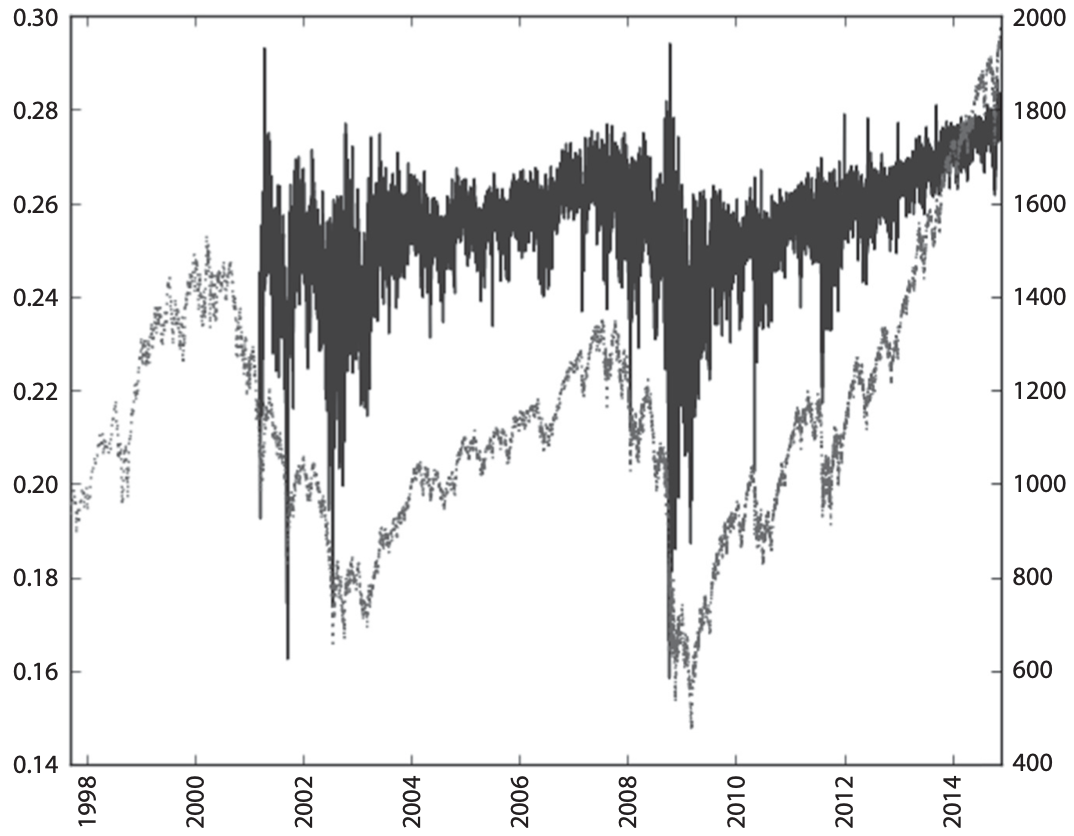
\includegraphics[scale=0.35]{/intro/fracdifffixedwidthwind}
\caption{Fractional differentiation controlling for weight loss with expanding and fixed-width window}
\end{figure}

\begin{method} \hlt{Expanding Window}\\
Given time series $T$ with real observations $\{X_t\}_{t = 1, \ldots, T}$, for each $l$, the relative weight loss is defined as
\begin{equation}
\lambda_l = \sum\limits_{j=T-l}^T \abs{\omega_j} \Bigg/ \sum\limits_{i=0}^{T-1} \abs{\omega_i} \nonumber
\end{equation}
Given tolerance level $\tau \in [0,1]$, determine value $l^*$ such that $\lambda_{l^*} \leq \tau$ and $\lambda_{l^* + 1} > \tau$. This value $l^*$ corresponds to the first results $\{\tilde{X}_t \}_{t = 1, \ldots, l^*}$, where weight-loss is beyond acceptable threshold $\lambda_t > \tau$.\\
From Remark \ref{rmk:propfracdifffeat}, it is clear $\lambda_{l^*}$ depends on convergence speed of $\{\omega_k \}$, which in turn depends on $d \in [0,1]$.\\
For $d = 1, \omega_k = 0 \ \forall k > 1$, and $\lambda_l = 0 \ \forall l > 1$, hence it suffices to drop $\tilde{X}_1$.\\
As $d \rightarrow 0^+$, $l^*$ increases, and larger portion of initial $\{\tilde{X}_t \}_{t = 1, \ldots, l^*}$ needs to be dropped to keep the weight loss $\lambda_{l^*} < \tau$. Note that there will be negative drift caused by negative weights added to initial observations as window is expanded. By controlling for weight loss, negative drift is still substantial as $\{\tilde{X}_t \}_{t = l^* + 1, \ldots, T}$ are computed on an expanding window.
\end{method}

\begin{method} \hlt{Fixed-Width Window}\\
Drop weights after their modulus $\abs{\omega_k}$ decreases below a given threshold $\tau$. This is equivalent to finding the first $l^*$ such that $\abs{\omega_{l^*}} \geq \tau$ and $\abs{\omega_{l^* + 1}} \leq \tau$, setting a new variable $\tilde{\omega}_k$:
\begin{align}
\tilde{\omega_k} = 
\begin{cases}
\omega_k \ \ \ \ \text{if } k \leq l^* \\
0 \ \ \ \ \ \ \text{if } k > l^*
\end{cases}, \ \ \ \ \
\tilde{X}_t = \sum\limits_{k=0}^{l^*} \tilde{\omega}_k X_{t-k} \ \ \text{for } t = T- l^* + 1, \ldots, T \nonumber
\end{align}
Note that the same vector of weights is used across all estimates of $\{\tilde{X}_t \}_{t = l^*, \ldots, T}$, hence avoiding negative drift caused by expanding window's added weights.\\
Distribution has skewness and excess kurtosis from memory, but it is stationary.
\end{method}